\section{Experiments and Analysis}
%To validate our approach, we conduct empirical  evaluations on two real-world datasets. 
Our experiments aim to answer these:

\begin{itemize}
    \item \textbf{RQ1.} Can \name prevent intent-divergence by context-aware sample selection? 
    (Results in \S~\ref{sec:eval_intent})
    %
    \item \textbf{RQ2.} Can approximate EDA with \name still captures the final insights as the original?
    (Results in \S~\ref{sec:eval_insight})
    %
    \item \textbf{RQ3.} Can \name provide significant latency reduction while addressing RQ1 and RQ2?
    (Results in \S~\ref{sec:eval_latency})
\end{itemize}

\begin{comment}
\begin{itemize}
    \item \textbf{RQ1.} Can our approach effectively select the best down-sampling strategies to reduce the computational cost while still achieve high accuracy?
    
    
    \item \textbf{RQ2.} Are user intents well preserved in the sample selection during the sequential data exploration over time? 
    
    
    \item \textbf{RQ3.} Can our model training be properly terminated in the sequential data exploration, by capturing key takeaway insights?
    
\end{itemize}
\end{comment}

\begin{figure}[!t]
\centering
\begin{minipage}[t]{0.495\columnwidth}
\vspace{0pt}
% \begin{table}[]
\scalebox{0.65}{
\begin{tabular}{|l|l|l|}
\hline
\begin{tabular}[c]{@{}l@{}}Sampling \\ Strategy\end{tabular} & \begin{tabular}[c]{@{}l@{}}No. of \\ Rows\end{tabular} & \begin{tabular}[c]{@{}l@{}}Effective\\  SR\end{tabular} \\ \hline
Uni@1\%                                                      & 5232                                                   & 0.01                                                    \\ \hline
Uni@5\%                                                      & 26155                                                  & 0.05                                                    \\ \hline
Uni@10\%                                                     & 52312                                                  & 0.1                                                     \\ \hline
Sys@100                                                      & 5231                                                   & 0.01                                                    \\ \hline
Sys@20                                                       & 26154                                                  & 0.05                                                    \\ \hline
Sys@10                                                       & 52311                                                  & 0.1                                                     \\ \hline
Clus@1\%                                                     & 5230                                                   & 0.01                                                    \\ \hline
Clus@5\%                                                     & 26154                                                  & 0.05                                                    \\ \hline
Clus@10\%                                                    & 52306                                                  & 0.1                                                     \\ \hline
MinMax@5\%                                                   & 27202                                                  & 0.052                                                   \\ \hline
MaxSum@5\%                                                   & 25109                                                  & 0.048                                                   \\ \hline
KStrat1@2k                                                   & 14124                                                  & 0.027                                                   \\ \hline
KStrat1@10k                                                  & 28771                                                  & 0.055                                                   \\ \hline
KStrat1@20k                                                  & 57542                                                  & 0.11                                                    \\ \hline
KStrat2@2k                                                   & 9416                                                   & 0.018                                                   \\ \hline
KStrat2@10k                                                  & 25125                                                  & 0.048                                                   \\ \hline
KStrat2@20k                                                  & 47080                                                  & 0.09                                                    \\ \hline
Strat1@1\%                                                   & 5220                                                   & 0.01                                                    \\ \hline
Strat1@5\%                                                   & 26146                                                  & 0.05                                                    \\ \hline
Strat1@10\%                                                  & 52375                                                  & 0.1                                                     \\ \hline
Strat2@1\%                                                   & 5232                                                   & 0.01                                                    \\ \hline
Strat2@5\%                                                   & 26148                                                  & 0.05                                                    \\ \hline
Strat2@10\%                                                  & 52320                                                  & 0.1                                                     \\ \hline
Strat3@1\%                                                   & 5240                                                   & 0.01                                                    \\ \hline
Strat3@5\%                                                   & 26150                                                  & 0.05                                                    \\ \hline
Strat3@10\%                                                  & 52315                                                  & 0.1                                                     \\ \hline
Strat4@1\%                                                   & 5235                                                   & 0.01                                                    \\ \hline
Strat4@5\%                                                   & 26149                                                  & 0.05                                                    \\ \hline
Strat4@10\%                                                  & 52321                                                  & 0.1                                                     \\ \hline
\end{tabular}
}
\captionof{table}{Details of Samples generated on Flights Dataset}
\label{tab:flights_samples}
\end{minipage}%
\hfill
\begin{minipage}[t]{0.495\columnwidth}
\vspace{0pt}
\begin{minipage}[t]{1.0\columnwidth}
\begin{minipage}[t]{1.0\columnwidth}
\vspace{0pt}
\scalebox{0.65}{
\begin{tabular}{|l|l|l|}
\hline
\begin{tabular}[c]{@{}l@{}}Sampling \\ Strategy\end{tabular} & \begin{tabular}[c]{@{}l@{}}No. of \\ Rows\end{tabular} & \begin{tabular}[c]{@{}l@{}}Effective\\  SR\end{tabular} \\ \hline
Uni@1\%                                                      & 3242                                                   & 0.01                                                    \\ \hline
Uni@5\%                                                      & 16210                                                  & 0.05                                                    \\ \hline
Uni@10\%                                                     & 32419                                                  & 0.1                                                     \\ \hline
Sys@100                                                      & 3241                                                   & 0.01                                                    \\ \hline
Sys@20                                                       & 16209                                                  & 0.05                                                    \\ \hline
Sys@10                                                       & 32419                                                  & 0.1                                                     \\ \hline
Strat1@1\%                                                   & 3246                                                   & 0.01                                                    \\ \hline
Strat1@5\%                                                   & 16225                                                  & 0.05                                                    \\ \hline
Strat1@10\%                                                  & 32425                                                  & 0.1                                                     \\ \hline
Strat2@1\%                                                   & 3238                                                   & 0.01                                                    \\ \hline
Strat2@5\%                                                   & 16215                                                  & 0.05                                                    \\ \hline
Strat2@10\%                                                  & 32426                                                  & 0.1                                                     \\ \hline
Strat3@1\%                                                   & 3240                                                   & 0.01                                                    \\ \hline
Strat3@5\%                                                   & 16208                                                  & 0.05                                                    \\ \hline
Strat3@10\%                                                  & 32420                                                  & 0.1                                                     \\ \hline
Strat4@1\%                                                   & 3248                                                   & 0.01                                                    \\ \hline
Strat4@5\%                                                   & 16206                                                  & 0.05                                                    \\ \hline
Strat4@10\%                                                  & 32425                                                  & 0.1                                                     \\ \hline
\end{tabular}
}

\captionof{table}{Details of Samples generated on Housing Dataset}
\label{tab:housing_samples}
\end{minipage}
\begin{minipage}[t]{1.0\columnwidth}
\scalebox{0.65}{
\begin{tabular}{|l|l|l|}
\hline
\begin{tabular}[c]{@{}l@{}}Sampling \\ Strategy\end{tabular} & \begin{tabular}[c]{@{}l@{}}No. of \\ Rows\end{tabular} & \begin{tabular}[c]{@{}l@{}}Effective\\  SR\end{tabular} \\ \hline
Uni@1\%                                                      & 4266                                                   & 0.01                                                    \\ \hline
Uni@5\%                                                      & 21334                                                  & 0.05                                                    \\ \hline
Uni@10\%                                                     & 42670                                                 & 0.1                                                     \\ \hline
Sys@100                                                      & 4266                                                  & 0.01                                                    \\ \hline
Sys@20                                                       & 21334                                                & 0.05                                                    \\ \hline
Sys@10                                                       & 42669                                                  & 0.1                                                     \\ \hline
Strat1@1\%                                                   & 4267                                                   & 0.01                                                    \\ \hline
Strat1@5\%                                                   & 21336                                                  & 0.05                                                    \\ \hline
Strat1@10\%                                                  & 42672                                                  & 0.1                                                     \\ \hline
Strat2@1\%                                                   & 4235                                                   & 0.01                                                    \\ \hline
Strat2@5\%                                                   & 21330                                                  & 0.05                                                    \\ \hline
Strat2@10\%                                                  & 42664                                                  & 0.1                                                     \\ \hline
Strat3@1\%                                                   & 4235                                                   & 0.01                                                    \\ \hline
Strat3@5\%                                                   & 21340                                                  & 0.05                                                    \\ \hline
Strat3@10\%                                                  & 42667                                                  & 0.1                                                     \\ \hline
Strat4@1\%                                                   & 4237                                                   & 0.01                                                    \\ \hline
Strat4@5\%                                                   & 21367                                                  & 0.05                                                    \\ \hline
Strat4@10\%                                                  & 42673                                                  & 0.1                                                     \\ \hline
\end{tabular}
}

\captionof{table}{Details of Samples generated on Income Dataset}
\label{tab:income_samples}
\end{minipage}
% \end{table}
\end{minipage}
\end{minipage}
\end{figure}


\subsection{Experimental Setup}
All experiments used a 32 core Intel(R)Xeon(R) CPU E5-2686 with 4 Tesla V100-SXM2 GPU(s). Model and implementation details are in supplement \ref{apps:model_implementation}.

\noindent\textbf{Datasets.}
%
%\sm{Add reference for each of the datasets}
%\noindent \textbf{Flights Data:}
Table~\ref{tab:dataset} summarizes the popular and public datasets: Flight~\cite{Flights} (also used by \cite{atena2020sigmod}), Housing~\cite{Housing} and Income~\cite{Income}
%Flights data contains records of past flights with attributes such as origin airport, destination airport, delay reason, etc.
%Housing data contains price records of houses with attributes like, area, #bedrooms, etc. 
%
%We use around $\sim 600k$ rows from this da
%This dataset contains records of past flights with attributes such as origin airport, destination airport, delay reason, etc. This dataset was  and we use their simulator to generate sequences as close to human analyst as possible. 
%We use around $\sim 500k$ rows from this dataset to train the simulator. Then 6000 unique sequences are generated for this dataset by the simulator and we train our RL agent using two strategies. In the first, we train the RL agent on all generated sequences and in the second, we holdout a set of 1200 sequences and train our RL agent on remaining 4800 sequences.
%\noindent \textbf{Taxi Data:}
%Taxi dataset~\cite{} is another public dataset that contains records of NYC taxi trips with attributes like, passenger count, trip duration, etc. 
%We use around $\sim 600k$ rows from this dataset for the simulator and generate X unique sequences, out of which Y are heldout for training the RL agent using second strategy.
%
%\noindent \textbf{Housing Data:} 
%Housing dataset is another public dataset that contains records of XXX. It has attributes like, X, Y, Z, etc. We use around $\sim 500k$ rows from this dataset for the simulator and generate A unique sequences, out of which B are heldout for training the RL agent using second strategy.




\noindent\textbf{Actions}
%
In total we use 29 actions based on 6 sampling strategies and corresponding parameter combinations as presented in Table~\ref{tab:actions}.
Effective SR denotes the sampling rate defined as total \# rows in the sample / \# rows in the full data. Table~\ref{tab:flights_samples},~\ref{tab:housing_samples},~\ref{tab:income_samples} show the effective sampling rate and the number of rows for different samples for each dataset.
% For stratified samples, we follow the approach proposed by~\cite{agarwal2013blinkdb} that extracts query-column-sets (QCS) from the historical queries used on the full dataset and create stratified samples for the set of QCS that covers 90\% of historical queries. 
%E.g., the QCS for stratified sample for following query would be [month, carrier]. 
%[month, origin, carrier]
%
%\tong{may make the following left aligned}
\begin{comment}
{\footnotesize 
\noindent\texttt{\textcolor{blue}{SELECT} carrier, \textcolor{blue}{AVG}(delay)
\textcolor{blue}{FROM} Data \\
\textcolor{blue}{WHERE}
month\textcolor{blue}{=}"JAN" 
%\textcolor{blue} {AND}
%origin\textcolor{blue}{=}"JFK"
\textcolor{blue}{GroupBY} carrier 
}
}
\end{comment}
%

% \begin{table}[]
% \scalebox{0.7}{
% \begin{tabular}{|l|l|l|l|l|l|}
% \hline
%                                 & \begin{tabular}[c]{@{}l@{}}EUD \\ (Zeta=0.25)\end{tabular} & \begin{tabular}[c]{@{}l@{}}EUD\\  (Zeta=0.5)\end{tabular} & \begin{tabular}[c]{@{}l@{}}\% \\ conversion\end{tabular} & 4.5    & 4.6    \\ \hline
% ApproxEDA                       & 0.0433                                                     & 0.2249                                                    & 0.0781                                                   & 0.0578 & 0.8507 \\ \hline
% ApproxEDA - R\_Term             & 0.0469                                                     & 0.2006                                                    & 0.0910                                                   & 0.0511 & 1.111  \\ \hline
% ApproxEDA - R\_Term - R\_Intent & 0.0777                                                     & 0.1904                                                    & 0.0903                                                   & 0.0399 & 1.3471 \\ \hline
% BlinkDB                         & 0.0593                                                     & 0.2336                                                    & 0.0865                                                   & 0.0333 & 0.5145 \\ \hline
% Uniform                         & 0.0533                                                     & 0.1941                                                    & 0.089                                                    & 0.0514 & 0.957  \\ \hline
% CI\_Greedy                      & 0.0854                                                     & 0.1992                                                    & 0.097                                                    & 0.0340 & 0.4821 \\ \hline
% CI\_Time\_Greedy                & 0.128                                                      & 0.2435                                                    & 0.135                                                    & 0.0085 & 0.6347 \\ \hline
% \end{tabular}
% }
% \captionof{table}{Results on the flights dataset}
% \label{tab:flight_results}
% \end{table}

% \begin{table}[]
% \scalebox{1}{
% \begin{tabular}{|l|l|l|}
% \hline
%           & Relative Distance & Relative IQCRec \\ \hline
% \name     & 1                 & 1               \\ \hline
% BlinkDB   & 1.37              & 0.58            \\ \hline
% CIGreedy  & 1.97              & 0.59            \\ \hline
% Uni@10\% & 1.23              & 0.89            \\ \hline
% Uni@1\%  & 1.79              & 0.61            \\ \hline
% \end{tabular}
% }
% \captionof{table}{Results on the flights dataset}
% \label{tab:flight_results}
% \end{table}

% \begin{table}[]
% \scalebox{1}{
% \begin{tabular}{|l|l|l|}
% \hline
%           & Relative Distance & Relative IQCRec \\ \hline
% \name     & 1                 & 1               \\ \hline
% BlinkDB   & 1.19              & 0.92            \\ \hline
% CIGreedy  & 0.64              & 0.92            \\ \hline
% Uni@10\% & 0.94              & 0.83            \\ \hline
% Uni@1\%  & 1.22              & 0.45            \\ \hline
% \end{tabular}
% }
% \captionof{table}{Results on the housing dataset}
% \label{tab:housing_results}
% \end{table}

\begin{figure*}[!t]
\begin{minipage}[t]{0.70\textwidth}
\centering
\begin{minipage}[t]{0.32\textwidth}
\begin{subfigure}{\textwidth}
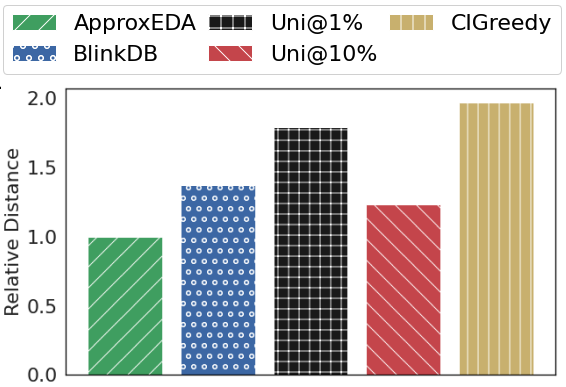
\includegraphics[width=1\linewidth]{LaTeX/figures/flights_eud.png}
\caption{Flights Dataset}
\end{subfigure}
\begin{subfigure}{\textwidth}
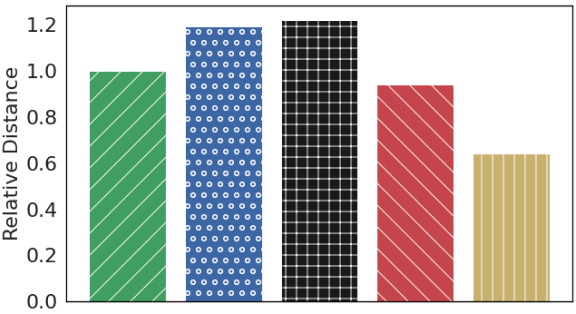
\includegraphics[width=1\linewidth]{LaTeX/figures/housing_eud.png}
\caption{Housing Dataset}
\end{subfigure}
\begin{subfigure}{\textwidth}
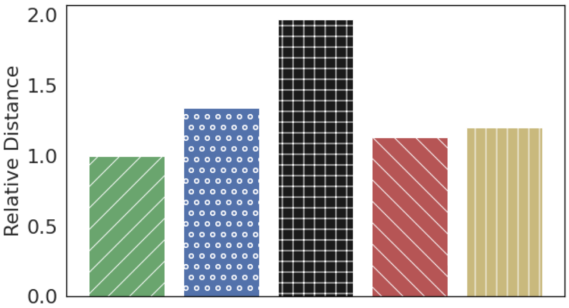
\includegraphics[width=1\linewidth]{LaTeX/figures/income_eud.png}
\caption{Income Dataset}
\end{subfigure}
\caption{Intent Divergence: Euclidean distance between original intent distribution and methods using samples. Normalized w.r.t. \name. Lower is better.}
\label{fig:rel_dist_1}
\end{minipage}%
\hfill
\begin{minipage}[t]{0.32\textwidth}
\begin{subfigure}{1\textwidth}
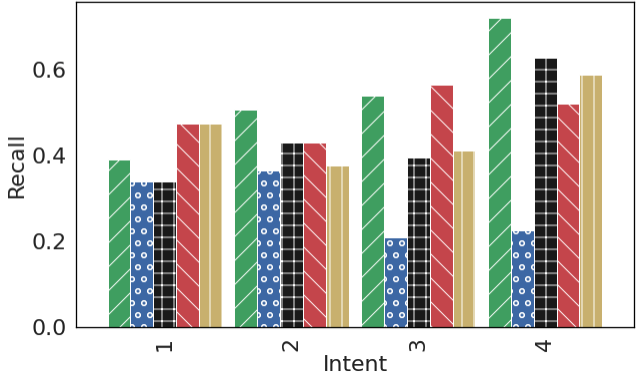
\includegraphics[width=1\linewidth]{LaTeX/figures/flights_intent1.png}
\caption{Flights Dataset}
\end{subfigure}
\begin{subfigure}{\textwidth}
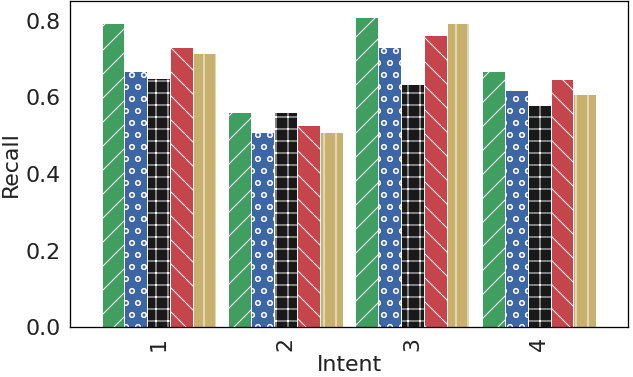
\includegraphics[width=1\linewidth]{LaTeX/figures/housing_intent.png}
\caption{Housing Dataset}
\end{subfigure}
\begin{subfigure}{\textwidth}
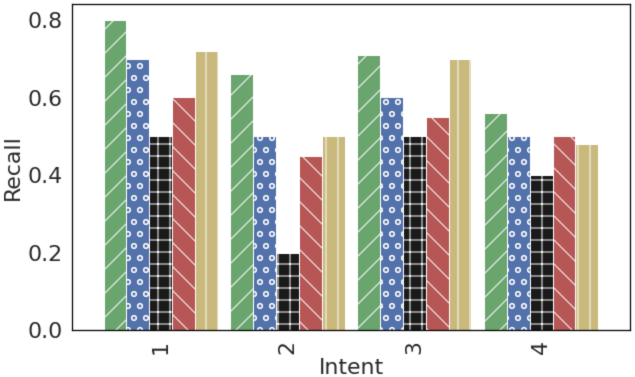
\includegraphics[width=1\linewidth]{LaTeX/figures/income_intent.png}
\caption{Income Dataset}
\end{subfigure}
\caption{Insight Preservation: Recall of the top 5 resulting rows at the end of analysis sequence compared to results from full data, across various intents. Higher is better.}
\label{fig:recall_5}
\end{minipage}%
\hfill
\begin{minipage}[t]{0.32\textwidth}
\centering
\begin{subfigure}{\textwidth}
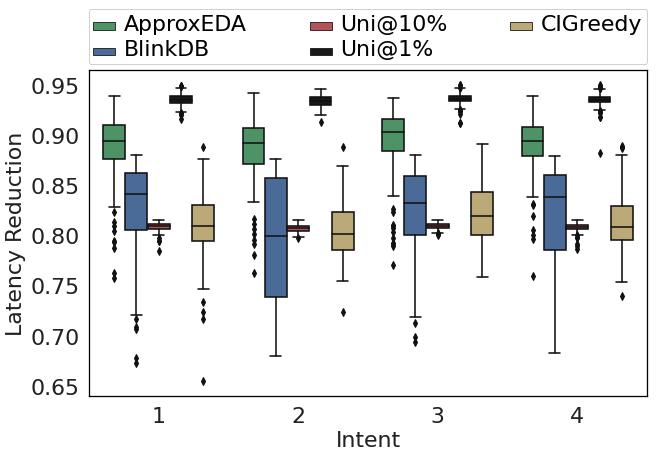
\includegraphics[width=1\linewidth]{LaTeX/figures/flight_lat.png}
\caption{Flights Dataset}
\end{subfigure}
\begin{subfigure}{\textwidth}
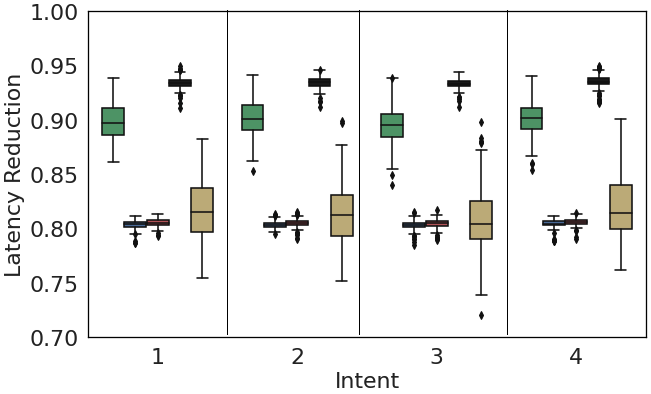
\includegraphics[width=1\linewidth]{LaTeX/figures/housing_lat_new.png}
\caption{Housing Dataset}
\end{subfigure}
\begin{subfigure}{\textwidth}
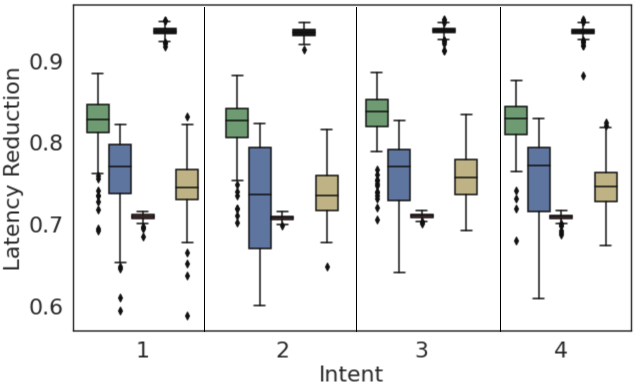
\includegraphics[width=1\linewidth]{LaTeX/figures/income_lat.png}
\caption{Income Dataset}
\end{subfigure}
\caption{The fraction of time saved by queries to run on the sampled dataset when using different models.
     Higher is better.}
     \label{fig:latency_reduction}
\end{minipage}%
%\hfill
\end{minipage}
\hfill
\begin{minipage}[t]{0.29\textwidth}
\centering
\begin{minipage}[t]{1.0\textwidth}
\centering
%\begin{table}
%\begin{center}
\scalebox{0.70}{
 \begin{tabular}[t]{|l|l|l|l|}
    \hline
    {Dataset} & {\# rows in full data} & {Unique sequences} \\
    \hline
    {Flights} & {5231403} & {10695}\\
    \hline
    {Housing} & {324196} & {6016} \\
    \hline
    {Income} & {426753} & {4032} \\
    \hline
    \end{tabular}
    }
 \captionof{table}{Dataset and EDA sequences}
 \label{tab:dataset}
%\end{center}
%\end{table}
\end{minipage}
\begin{minipage}[t]{1.0\textwidth}
\centering
 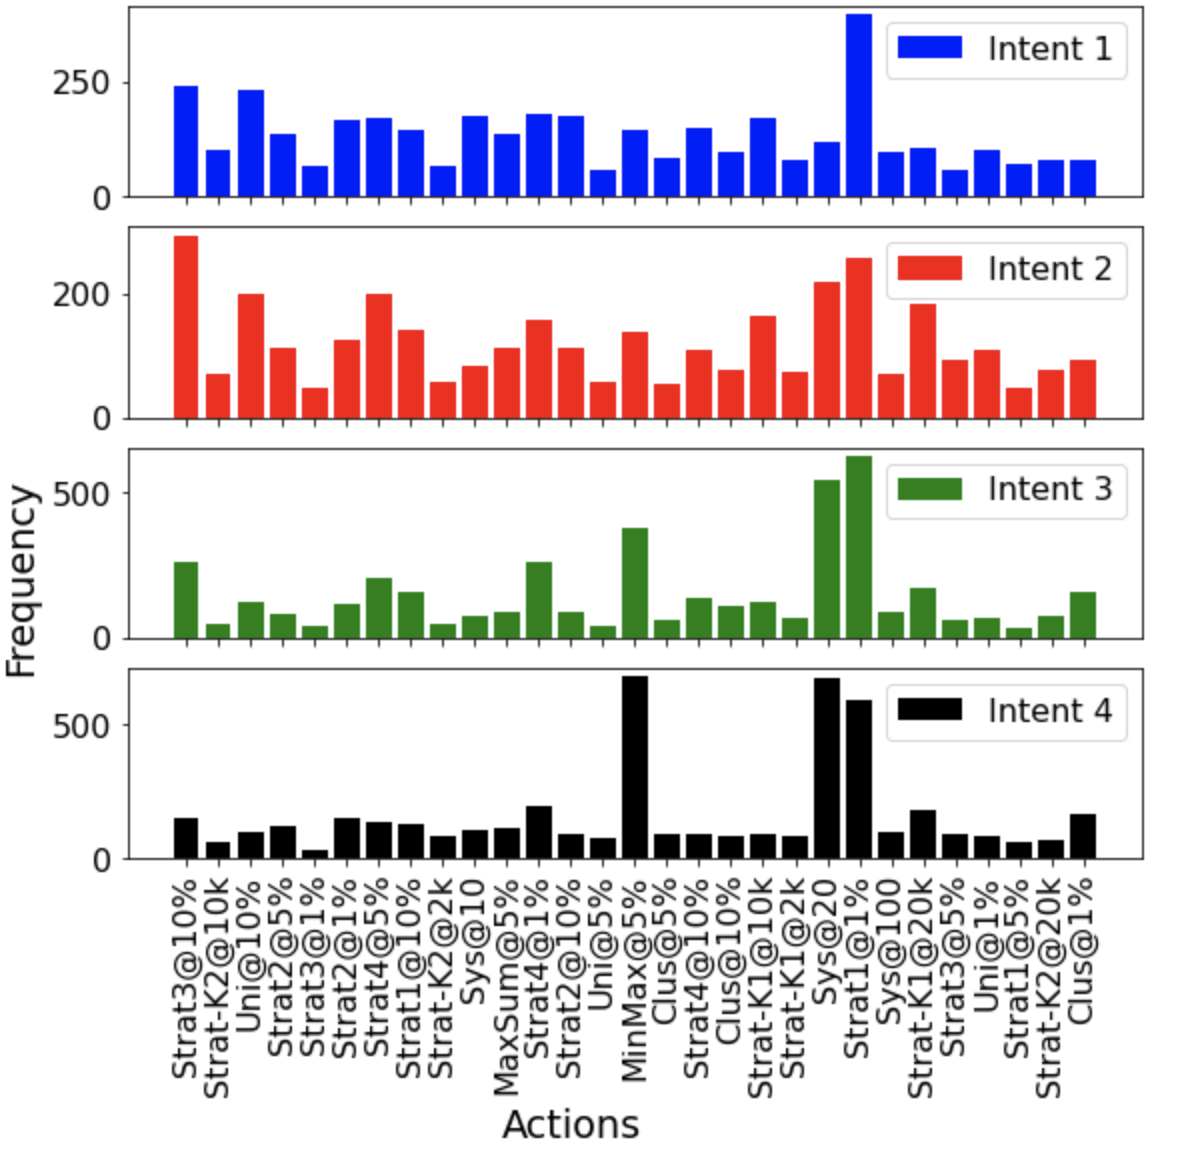
\includegraphics[width=\textwidth]{LaTeX/figures/intent_actions2.png}
      \caption{Frequency of different actions taken by \name for different intents.}
      \label{fig:action_usage}
 \end{minipage}
\end{minipage}
\vspace{-0.5em}
\end{figure*}


% \begin{figure*}[!t]
% \begin{minipage}[t]{0.4\textwidth}
% \begin{subfigure}{1\textwidth}
% \includegraphics[width=1.0\linewidth]{LaTeX/figures/Frame 50.png}
% \end{subfigure}
% \caption{Intent Divergence: Euclidean distance between original intent distribution and methods using samples. Normalized w.r.t. \name. Lower is better.}
% \label{fig:rel_dist_1}
% \end{minipage}%
% \hfill
% \begin{minipage}[t]{0.59\textwidth}
% \begin{subfigure}{1.0\textwidth}
% \includegraphics[width=1\linewidth]{LaTeX/figures/Frame 49 (2).png}
% \end{subfigure}
% % \begin{subfigure}{.3\textwidth}
% % 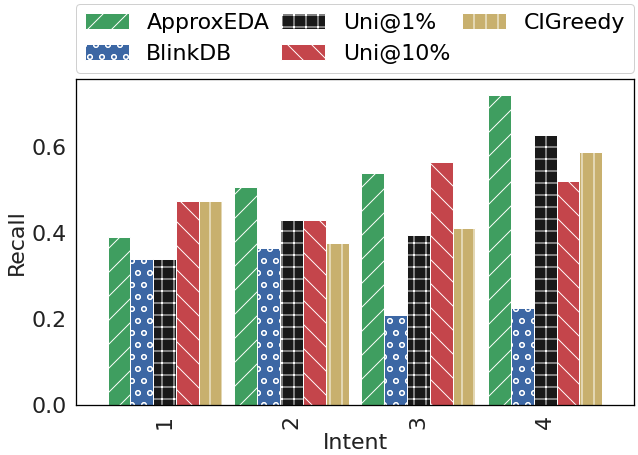
\includegraphics[width=1\linewidth]{LaTeX/figures/flights_5.png}
% % \caption{Flights Dataset}
% % \end{subfigure}
% % \begin{subfigure}{.3\textwidth}
% % 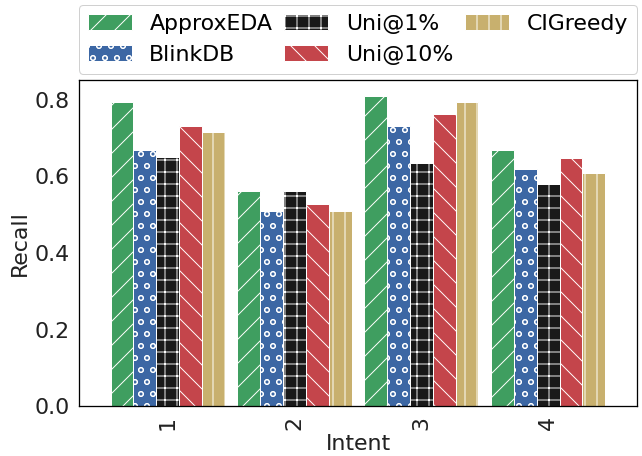
\includegraphics[width=1\linewidth]{LaTeX/figures/housing_5.png}
% % \caption{Housing Dataset}
% % \end{subfigure}
% % \begin{subfigure}{.3\textwidth}
% % 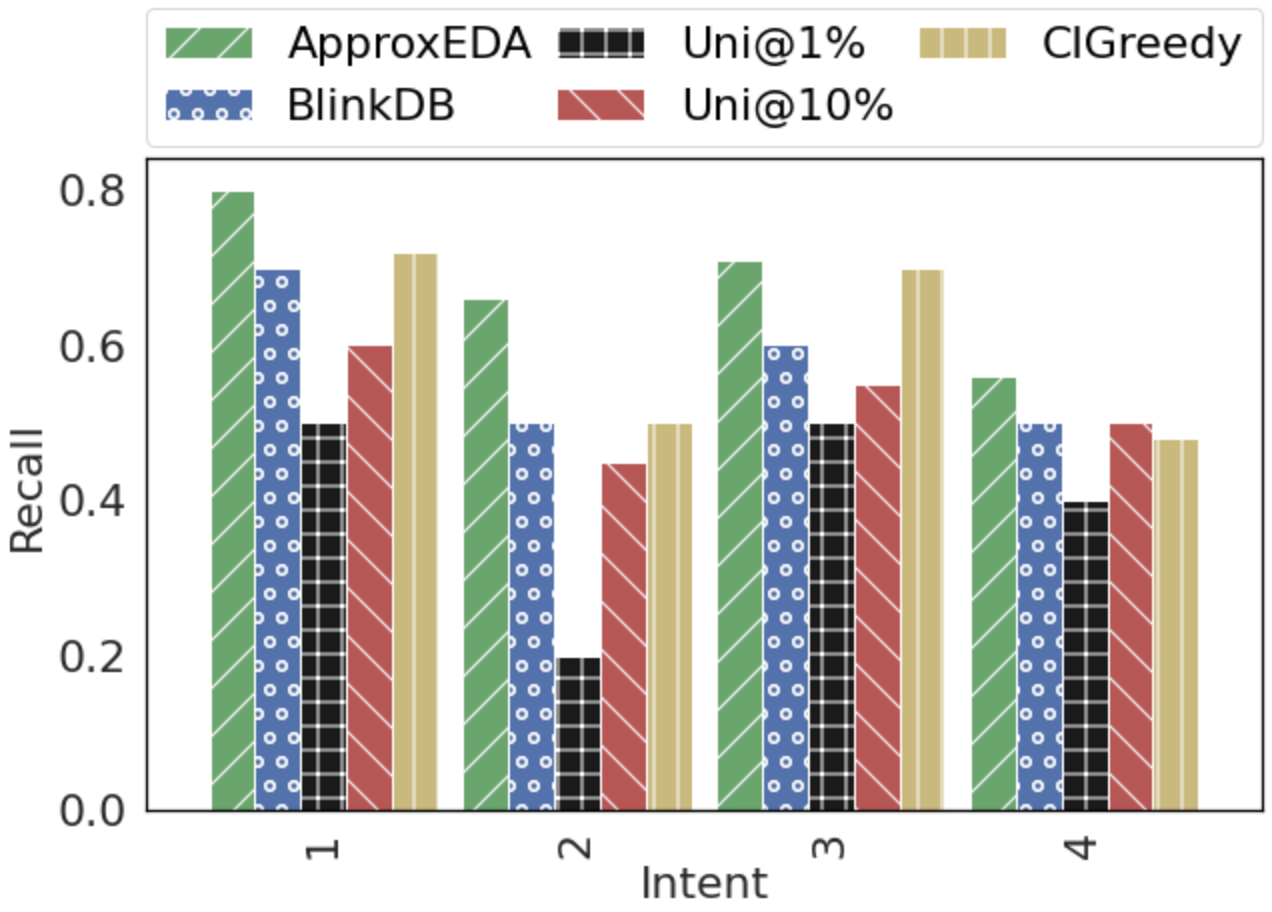
\includegraphics[width=1\linewidth]{LaTeX/figures/intent_preserve_income.png}
% % \caption{Income Dataset}
% % \end{subfigure}
%      \caption{Insight Preservation: Recall of the top 5 resulting rows at the end of analysis sequence compared to results from full data, across various intents.
%      Higher is better.}
%      \label{fig:recall_5}
% \end{minipage}
% \vspace{-1.0em}
% \end{figure*}


% \begin{table}[]
% \scalebox{1}{
% \begin{tabular}{|l|l|l|l|}
% \hline
%                  & \begin{tabular}[c]{@{}l@{}}EUD \\ (Zeta=0.25)\end{tabular} & 4.5  & 4.6   \\ \hline
% ApproxEDA        & 0.031                                                      & 0.12 & 0.728 \\ \hline
% BlinkDB          & 0.037                                                      & 0.11 & 0.73  \\ \hline
% Uniform          & 0.029                                                      & 0.10 & 0.45  \\ \hline
% CI\_Greedy       & 0.020                                                      & 0.11 & 0.40  \\ \hline
% CI\_Time\_Greedy & 0.022                                                      & 0.11 & 0.74  \\ \hline
% \end{tabular}
% }
% \captionof{table}{Results on the housing dataset}
% \label{tab:housing_results}
% \end{table}



\noindent\textbf{Baselines.}
%We compare with the following baselines:
\begin{itemize}
\item \noindent\textbf{\blink:}
%This is a state-of-the-art technique~\cite{agarwal2013blinkdb} for selecting a sample to get an approximate result for each individual query. 
\blink~\cite{agarwal2013blinkdb} attempts to minimize error for each query by selecting the stratified-sample that has the best overlap for QCS (explained before) of the
incoming query to be executed. 
When no overlap with stratified samples, we use 1\% uniform sample. 
%It does not have a notion of the intent or EDA sequences. 

\item \noindent\textbf{\greedy:}
We develop another intelligent baseline that first calculates a confidence interval (CI) for aggregate value requested by the incoming query on all the available samples (using a closed form formulation from~\cite{mozafari2015handbook}). 
Then chooses sample with the tightest CI at 95\% (i.e. indicating more confidence in the result).

\item \noindent{Uni@10\% and Uni@1\%:}
We compare our results with two other baselines where the agent always chooses a Uniform 10\% sample and Uniform 1\% sample respectively.
\end{itemize}

\noindent\textbf{Parameters.}
We use $K=4$ intents from BTM as it maximizes overall UCI score. Appendix~\ref{apps:intent_identification} and Figure~\ref{fig:intent_cluster} shows the clusters and UCI scores. We use values of $\beta$ and $\gamma$ as 1 to provide equal weightage to rewards after scaling them.
%\tong{this sentence may be moved to the experiment section?}

\subsection {Evaluation Methodology}
\label{sec:evaluation}
\vspace{-0.1em}
%
%While generation of these EDA sequences, we fix the first $k=3$ queries\footnote{We found usually first 3 or 4 queries and corresponding visualization set the experience analysts on a particular EDA flow particular initial queries From our domain experience}  
%\sm{Revisit this k=3 evaluation setup.}
%
%Note: only \name has the ability to do this selection in an intent-aware manner.
%
%\sm{Following may go in the ablation study.}
%For \name we present two sets of results: \textbf{seen} and \textbf{unseen}, when the held-out set is also used to learn the intents, and when it is not, respectively.



\begin{comment}
\begin{table}
\scalebox{0.8}{
 \begin{tabular}[ht!]{|l|l|l|c|}
    \hline
    {Sample Name} & {Short Name} & {Parameters} & {Effective SR}\\
    \hline
    {Uniform} & {Uni@$\tau$} & {$\tau$= [0.01, 0.05, 0.1]} & {[0.01, 0.05, 0.1]} \\
    \hline
    {Systematic} & {Sys@$k$} & {$k$= [100, 20, 10]} & {0.01, 0.05, 0.1]} \\
    \hline
    {Proportional stratified} & {Strat@$\tau$} & {$\tau$= [0.01, 0.05, 0.1]} & {[0.01, 0.05, 0.1]} \\
    \hline
    {At most $K$ stratified} & {Strat-K@$k$} & {$K$= [0.1]} & {[0.1]} \\
    \hline
    {Cluster} & {Clus@$k$} & {$k$= 10, $\tau$= [0.01, 0.05, 0.1]} & {[0.01, 0.05, 0.1]} \\
    \hline
    {Diversity} & {Div@$k$} & {$k$= 0.1*$|T|$} & {[0.1]} \\
    \hline
    \end{tabular}
    }
 \captionof{table}{Samples used as actions \sm{Make sure these parameter notations are explained in Sec-2.}}
 \label{tab:actions}
\end{table}
\end{comment}

\noindent\textbf{EDA Interactions using ATENA.}
%This is because data on which users perform such analyses are often proprietary. Moreover, the process being highly interactive and performed by proficient analysts, curating such a large volume of such data can be prohibitively costly. 
%
%We are the first to look at this problem of how to protect analysis intent divergence while using samples to speed up interactions. 
%As the problem of intent-divergence during EDA was not explored before, 
There are no public datasets available that combines both exploratory insight generation query sequences and the corresponding results on a given data that is also publicly available. 
Moreover, similar to many other interactive scenarios, such as conversational recommender systems \cite{christakopoulou2016towards}, dialog systems \cite{shi2019build,takanobu2020multi} and dialog-based interactive image retrieval \cite{guo2018dialog,yu2019visual}, a major challenge in the evaluation is that we need to have access to user reactions to any possible results returned by the system, which are exhaustive to collect in practice. Therefore, similar to \cite{christakopoulou2016towards,guo2018dialog,yu2019visual,shi2019build}, we adopt a setting where the user reactions are generated by simulators as surrogates for real users.
We overcome this by using an EDA simulator from prior work~\cite{atena2020sigmod}, called ATENA that is trained using real analysis sequences from expert analysts, which uses high-level statistical characteristics 
% (e.g. entropy, skew, \# unique categories etc.) 
of the data along with its schema structure 
% (e.g. numerical, categorical, primary-key column information) 
to generate realistic analysis sequence patterns similar human experts with various implicit intents~\cite{atena2020sigmod}.
%Similar to a real user, ATENA also formulates the next SQL query based on the previous set of queries that were run along with the corresponding results or displays (e.g. groups of rows from a \texttt{SELECT} or \texttt{GroupBy} query). Evaluations of ATENA show that the resulting query ordering and their coherence in the EDA sequences closely match with interactive analysis done by human experts on the same target dataset.  
%
%Specifically, 
%We use ATENA to both generate ideal exploratory sessions when no approximations through sampling is used, as well as to create interactive environment when samples are used and selected by our proposed RL-agent.
%
%This approach is similar to several prior works that used a simulator to evaluate a solution in an interactive setup~\cite{}. 
%\sm{Tong please specify few paper}.
%
%When training machine learning models of interactive systems, we usually use user simulators \citep{liu2018dialogue,shi2019build,guo2018dialog}.
%
%Similar to many other interactive scenarios, such as conversational recommender systems \cite{christakopoulou2016towards}, dialog systems \cite{shi2019build,takanobu2020multi} and dialog-based interactive image retrieval \cite{guo2018dialog,yu2019visual}, a major challenge in the evaluation is that we need to have access to user reactions to any possible results returned by the system, which are exhaustive to collect in practice. Therefore, similar to \cite{christakopoulou2016towards,guo2018dialog,yu2019visual,shi2019build}, we adopt a setting where the user reactions are generated by simulators as surrogates for real users.
For each of the datasets, we train this simulator following the methodology described in \cite{atena2020sigmod}.
Then we use this trained stochastic simulator to generate data exploration sessions which constitute sequence of queries and corresponding results or visualizations. 
For each dataset several such unique sequences can be generated by the simulator using multiple runs and is summarized in Table~\ref{tab:dataset}.
For each dataset, we set aside $1k$ sequences generated by the simulator using full data as held-out set for evaluations.
For \name and the baselines, we also generate $1k$ sequences by letting these methods interact with the simulator where for each query of the EDA, these methods select the optimal samples using their respective algorithms. 
%
Each of the sequences generated from any of the methods are fed into the BTM model to get the probability distribution of intents over the topics.

%\subsubsection{Metrics}

\subsection{Evaluation:Intent Divergence (RQ1)}
\label{sec:eval_intent}

We evaluate \name compared to the baselines in preserving the intent distributions (distribution of EDA interaction sequences over topic-models) of the original EDA sequences created without using any samples for approximations. 
%
In Figure ~\ref{fig:rel_dist_1} we present Euclidean Distance (ED) (normalized w.r.t. \name) between the intent distributions resulting from one of the baselines and from original unapproximated scenario. 
Lower ED is desirable as it indicates better matching of intent distribution. 
We can see that for Flights and Income, \name is best in preserving the distribution. 
For Housing it {Uni@10\%} (uniform sample at 10\%) and \greedy does better. 
This is because both {Uni@10\%} (uniform sample at 10\%) and \greedy ends up choosing large overall sample sizes, and hence less information loss and approximation error.  
However, in the following \S~\ref{sec:eval_latency} and associated latency improvement plot in Figure~\ref{fig:latency_reduction}, we see that such use of large samples makes these methods extremely poor for latency reduction and defeats the purpose of using samples to speed up interactivity. 
Supplement (\textbf{A.1}) provides the exact number of rows corresponding to each samples (actions) created by various sampling strategies.
%
%
%Since the EDA simulator we use is stochastic and \name intervenes with the simulator by providing samples to run the queries instead of the full original data --- it is not possible to exactly compare an EDA interaction sequence created while using \name with a particular \textit{ground truth sequence}.
%
%

\begin{comment}
The metric finally for n such sequences is the,
\begin{equation}
    Intent Accuracy = \frac{No. of correctly identified intents}{Total no. of sequences}
\end{equation}

\tong{Please follow notations from existing papers, instead of starting from scratch for the above equation.}

We evaluate how well the final insight of the EDA is preserved in addition to preserving the intent distribution. 
To do this, we define a metric Intent-Query-Coherence (IQC) that calculates the probability of a query, given its intent as follows:
\begin{equation}
    IQC(q_i | intent) = average(P(q_i | intent))
\end{equation}
across the test samples for a specified intent.

For this we use the last $k=2$ queries of the EDA sessions as representation of the \textit{final insight} that an analyst would use as key takeaways.

For last two queries generated by \name and baselines,
we calculate $X = \frac{IQC(Q_{L}) + IQC(Q_{L-1})}{2}$ the \textit{IQC} metric using $\argmax(P(S)$ as the given intent $I$ based on the resulting sequence $S$.
$L$ length of the EDA sequence.

Then we calculate a metric for final insight recall (FIR) for each method as:
Avg-over-each-generated-sequence($X$*Recall for results $Q_{l}$ and $Q_{l-1}$ over all sequences from $I$).

Recall is calculated over with k=3-5-10 rows in the result for each of the queries.
Precision is not important.

\end{comment}

\begin{figure*}[t!]
\begin{minipage}[t]{0.495\textwidth}
%\begin{table}[]
\scalebox{0.67}{
\begin{tabular}{|l|l|l|llll|}
\hline
\multirow{2}{*}{Model} & \multirow{2}{*}{\begin{tabular}[c]{@{}l@{}}Relative\\ ED\end{tabular}} & \multirow{2}{*}{\begin{tabular}[c]{@{}l@{}}Latency\\ Reduction\end{tabular}} & \multicolumn{4}{c|}{Overall Mean Recall}                                                                         \\ \cline{4-7} 
                       &                                                                              &                                                                              & \multicolumn{1}{l|}{Intent 1} & \multicolumn{1}{l|}{Intent 2} & \multicolumn{1}{l|}{Intent 3} & Intent 4 \\ \hline
\name                  & \textbf{1}                                                                            & 0.89                                                                         & \multicolumn{1}{l|}{0.32}     & \multicolumn{1}{l|}{\textbf{0.74}}     & \multicolumn{1}{l|}{0.29}     & 0.63     \\ \hline
\name - $R_{term}$     & 1.08                                                                         & \textbf{0.92}                                                                         & \multicolumn{1}{l|}{\textbf{0.39}}     & \multicolumn{1}{l|}{0.60}     & \multicolumn{1}{l|}{\textbf{0.32}}     & 0.38     \\ \hline
\name - $R_{intent}$   & 1.36                                                                         & 0.91                                                                         & \multicolumn{1}{l|}{0.31}     & \multicolumn{1}{l|}{0.57}     & \multicolumn{1}{l|}{0.30}     & 0.35     \\ \hline
\name - $R_{latency}$  & 1.12                                                                         & 0.83                                                                         & \multicolumn{1}{l|}{0.28}     & \multicolumn{1}{l|}{0.68}     & \multicolumn{1}{l|}{0.29}     & \textbf{0.68}     \\ \hline
\end{tabular}
}
\captionof{table}{Impact of different components of rewards.}
\label{tab:ablation_results}
%\end{table}
\end{minipage}%
\hfill
\begin{minipage}[t]{0.49\textwidth}
%\begin{table}[]
\scalebox{0.66}{
\begin{tabular}{|l|l|l|llll|}
\hline
\multirow{2}{*}{Action Space}                                             & \multirow{2}{*}{\begin{tabular}[c]{@{}l@{}}Relative\\ ED\end{tabular}} & \multirow{2}{*}{\begin{tabular}[c]{@{}l@{}}Latency\\ Reduction\end{tabular}} & \multicolumn{4}{c|}{Overall Mean Recall}                                                                         \\ \cline{4-7} 
                                                                          &                                                                              &                                                                              & \multicolumn{1}{l|}{Intent 1} & \multicolumn{1}{l|}{Intent 2} & \multicolumn{1}{l|}{Intent 3} & Intent 4 \\ \hline
Only Uniform                                                              & 1.34                                                                         & \textbf{0.90}                                                                         & \multicolumn{1}{l|}{\textbf{0.41}}     & \multicolumn{1}{l|}{0.60}     & \multicolumn{1}{l|}{0.28}     & 0.48     \\ \hline
Uniform + Stratified                                                      & \textbf{0.85}                                                                         & 0.84                                                                         & \multicolumn{1}{l|}{0.34}     & \multicolumn{1}{l|}{0.58}     & \multicolumn{1}{l|}{\textbf{0.30}}     & 0.65     \\ \hline
\begin{tabular}[c]{@{}l@{}}Uniform + Stratified \\ + Cluster\end{tabular} & 1.12                                                                         & \textbf{0.90}                                                                         & \multicolumn{1}{l|}{\textbf{0.41}}     & \multicolumn{1}{l|}{0.60}     & \multicolumn{1}{l|}{\textbf{0.30}}     & \textbf{0.66}     \\ \hline
All Samples                                                               & 1                                                                            & 0.89                                                                         & \multicolumn{1}{l|}{0.32}     & \multicolumn{1}{l|}{\textbf{0.74}}     & \multicolumn{1}{l|}{0.29}     & 0.63     \\ \hline
\end{tabular}
}
\captionof{table}{Ablation study: variations of action space.}
\label{tab:sample_results}
%\end{table}
\end{minipage}
\vspace{-0.8em}
\end{figure*}


\vspace{-0.2em}
\subsection{Evaluation: Insight Preservation (RQ2)}
\label{sec:eval_insight}
\vspace{-0.2em}

We evaluate how well the final insight of the EDA is preserved in addition to preserving the intent distribution.
Analysts usually derive insights at the end of each analysis sequence, using the outcome of the final few queries.
Since we do not have explicit labels about whether user actually received satisfactory insights at the end, we calculate a recall value based on results of row obtained from
different sampling based methods w.r.t. results obtained from use of full data.
To calculate this recall, we use top $k=5$ result rows obtained from last 2 queries from each of the analysis sequence -- a thumb rule we understood by talking to experts.

{\footnotesize
\begin{equation}
\label{recall_equation}
    Recall_{Intent=I} = \frac{|\bigcup_{i=1}^{n}M(Q_{i}) \cap \bigcup_{j=1}^{m}M(O_{j})|}{|\bigcup_{j=1}^{m}M(O_{j})|} , {Q_{i},O_{j}} \in I
\end{equation}
}

where $Q_i$ refers to the generated sequence, $O_j$ refers to the sequence generated on full data and $M(Q_i)$ is the union of the top $k$ results of the last two queries of the sequence $Q_i$.

Please note: the intent distribution (\S~\ref{sec:eval_intent}) along with this final insight preservation, as a combination ensures that users' do not diverge from their analysis workflow.  
This is because there can be hypothetical solutions that might directly match the results from last few queries, without replicating the intent of the analysis captured through the entire sequence of analysis. Even though, such a solution  would provide a high recall, but will fail to preserve the purpose of data exploration and associated understanding consumed by analysts~\cite{atena2020sigmod}. 
%
From Figure~\ref{fig:recall_5} we see that for 2 out of 4 intents for Flights data and all of the intents for Housing data and Income data, \name provides highest recall compared to the baselines. 
As explained in \S~\ref{sec:eval_intent}, the reason either {Uni@10\%} or \greedy sometimes provide higher recall because they end up choosing large sample sizes, which intern lead to much higher latency (Figure~\ref{fig:latency_reduction}). 
We also compute an \textit{overall recall} corresponding to all the results returned by the last 2 queries and illustrate in \ref{app:add_res}. 



\vspace{-0.2em}
\subsection{Evaluation:Latency Reduction (RQ3)}
\label{sec:eval_latency}
\vspace{-0.2em}

In Figure~\ref{fig:latency_reduction} we compare the latency improvement by \name compared to the other baselines. 
We compute the overall latency at a sequence level by summing up latency for each individual queries in that sequence. 
We calculate \% of reduction in sequence-level latency compared to the latency when each query execute against full data (y-axis: higher is better).
%
We show box-plots to show the distribution of values for each sequences, grouped by different intents. 
It can be observed that median sequence-level latency reduction for \name is almost 90\% (that is the analysis sequences take only $1/10^{th}$ of the original time.
%
Note: even though {Uni@1\%} provides most reduction as it always uses 1\% sample of the data irrespective of the context. 
Recall from Figure~\ref{fig:rel_dist_1} and ~\ref{fig:recall_5}, {Uni@1\%} is pretty bad in terms of preserving the intent distribution or the final insights. The combination of RQ1, RQ2 and RQ3 shows that \name's state can capture different context of sequential analysis and choose optimum trade-off space between statistical effectiveness of different samples vs. corresponding latencies.

 
% \tong{need some notations. Please follow notations from existing papers, instead of starting from scratch for the equation.}



\vspace{-0.2em}
\subsection{Qualitative Evaluation}
\vspace{-0.2em}
%
Due to space, in Appendix~\textbf{\ref{apps:qualitative_eval}} Figure~\ref{fig:real} we show a real EDA session with \name to illustrate in-spite of it selecting frugal samples at various points (e.g. Clus@1\%, Uni@5\% etc.), \name can mostly preserve the query structure, analysis sequence and final outcome/insight. 
In Figure~\ref{fig:action_usage} we show the variation of \name's choice of different actions (selection of samples) for 4 different intents identified for the Flights data across all the held out sequences.
We found that certain samples (e.g. MaxMin@5\%, Sys@20\%, Strat1@1\%) were predominantly chosen for certain intents (e.g. \#4). Intuition is that such samples can preserve representations of smaller groups better, which is necessary for that intent preservation.

\subsection{Ablation Study}
%
We conduct an ablation study to illustrate the effect of each component on the final metrics in Table~\ref{tab:ablation_results}.
The show Relative-ED, Latency-Reduction and Mean-Overall-Recall as the metric. We progressively remove one reward at a time and see the effect it has on the metrics. Comparing \name and \name - $R_{term}$ , we observe that the latency reduction increases. This is because $R_{latency}$ now has a greater impact on the total reward. However, this is accompanied by a sharp decrease in the Mean Recall value for Intent 2 and Intent 4 as this metric is highly dependant on $R_{term}$. The increase in mean recall for Intent 1 and Intent 3 is nominal.
%
Removing the $R_{intent}$, we notice that the model now performs worse on every metric except latency. This is because both Relative ED and Mean Recall are highly intent dependant and the lack of intent reward makes it difficult for model to learn a good enough distribution. The improvement in latency can be credited to the higher weight of the latency reward as seen in earlier the earlier case. 
%
We then verify the effect of removing $R_{latency}$. As expected, we observe that the latency reduction has largely dropped and thus the agent trained without $R_{latency}$ is free to choose larger samples in order to maximise the reward. We notice that, the model now  performs similar to \name and is better in terms of Metric Recall on Intent 4.
Table~\ref{tab:sample_results} shows sensitivity of \name w.r.t. to availability of different groups of sampling algorithms in its action space.

\begin{table}[th]
\tiny

\label{table:ablation_delta}
\begin{tabular}{|l|l|l|llll|}
\hline
\multicolumn{1}{|c|}{\multirow{2}{*}{\begin{tabular}[c]{@{}c@{}}Model \\ Parameter\end{tabular}}} & \multicolumn{1}{c|}{\multirow{2}{*}{Relative ED}} & \multicolumn{1}{c|}{\multirow{2}{*}{\begin{tabular}[c]{@{}c@{}}Latency \\ Reduction\end{tabular}}} & \multicolumn{4}{c|}{\begin{tabular}[c]{@{}c@{}}Mean Overall\\  Recall\end{tabular}}                                           \\ \cline{4-7} 
\multicolumn{1}{|c|}{}                                                                            & \multicolumn{1}{c|}{}                             & \multicolumn{1}{c|}{}                                                                              & \multicolumn{1}{c|}{Intent 1} & \multicolumn{1}{c|}{Intent 2} & \multicolumn{1}{c|}{Intent 3} & \multicolumn{1}{c|}{Intent 4} \\ \hline
$\delta =1$                                                                                         & 1                                                 & 0.89                                                                                               & \multicolumn{1}{l|}{0.32}     & \multicolumn{1}{l|}{0.74}     & \multicolumn{1}{l|}{0.29}     & 0.68                          \\ \hline
$\delta = 0$                                                                                        & 1.2                                               & 0.90                                                                                               & \multicolumn{1}{l|}{0.31}     & \multicolumn{1}{l|}{0.61}     & \multicolumn{1}{l|}{0.3}      & 0.42                          \\ \hline
\end{tabular}
\caption{Ablation study: Variation of $\delta$ in $R_{intent} = R_{dis} + \delta*R_{topic}$ (Ref. \S~\ref{sec:reward}).}
\label{tbl:ablation_delta}
\end{table}

We also do an ablation study on  $\delta$ and show the same in Table~\ref{tbl:ablation_delta}.
We observe that both components of our reward are important. Setting $\delta=0$ increases our relative distance between distributions. Although it reduces the latency, the gain is small. We also see that for various intents, our recall decreases significantly for Intent 2 and Intent 4. This is because setting $\delta=0$ removes the component that matches intent of the original sequence with the generated.

%\subsection{Discussion}
%\sm{Details/discussions on why the RL-based approach does better than baselines such as BlinkDB and others?
%
%It’s always an accuracy vs latency trade off, and the paper should motivate and demonstrate that the RL-based approach leads to more accuracy in less time compared to baselines.
%
%“The authors do not sufficiently discuss the downsides of an intent-aware sampling approach. For example, the proposed strategy introduces a bias towards, unlike its main competitors that sample uniformly at random. Consequently, it remains unclear whether the proposed method can estimate a truly exploratory user intent, as it will be more random (ln. 118). The introduced bias appears to be more problematic than the accumulated approximation error.”
%However, the query can be highly diverse. It means training a reliable policy in the proposed deep RL is hard by itself. Since the motivation of sampling is processing efficiency and in turn this paper aims to address the issues due to sampling, the impact of the RL must be evaluated



\begin{comment}

\subsubsection{Precision/Recall}
This captures the precision and recall numbers for the top $m$ groups in the result of last $k$ queries of the sequence. The analyst may reach the same state by different paths and the last $k$ queries are the most important for the exploration and we want the results to be as close as possible. \tong{need some notations. Please follow notations from existing papers, instead of starting from scratch for the  equation.}

\subsection{Results and Analysis}
\colorbox{yellow}{Experiment section 4:} 
\begin{itemize}
    \item Find a greedy baseline
    \item Find the closest paper and modify it to suit to our needs
    \item Find an evaluation metric and compare the following things on this metric:
        \begin{itemize}
            \item Greedy vs Published vs Our Method (best performing model) for 3 datasets
            \item Intent identification accuracy numbers for original vs fixed vs agent when first k queries out of n are fixed and rest are generated by simulator from these strategies.
            \item For a fixed sample, percentage savings over the original compared to some fixed strategies. 
            \item Ablation study experiment results
            \item Experiment with various RL algorithms like PPO/AUC and show the convergence properties.
            \item Look into what TBleu does and see if it can be useful
            \item Somehow fix last 2-3 queries and then compare
        \end{itemize}



\end{itemize}
\end{comment}